%\documentclass[xetex,mathserif,serif]{beamer}
\documentclass{beamer}
\renewcommand{\tiny}{\fontsize{4}{14}\selectfont}

\usepackage{hyperref}
\usepackage{fontspec} 
\usepackage{xunicode} %Unicode extras!
\usepackage{xltxtra} %Fixes 
\usefonttheme{professionalfonts}
\setmainfont{Linux Libertine O}
%\setmonofont[Scale=0.86]{DejaVu Sans Mono}
\setmonofont{Liberation Mono}
%\setromanfont{Silkscreen}
%\setsansfont{DejaVu Sans}
\setsansfont{Droid Sans}

\usepackage[final,expansion=true,protrusion=true,spacing=true,kerning=true]{microtype}
\usetheme{openlab} 
\setbeamertemplate{navigation symbols}{}
\usepackage{graphicx}

\title[Developers]{Open IT Lab} 
\author{Jarrell Waggoner} 
\institute[Open IT Lab] {Open IT Lab\\
  \medskip
      {\emph{waggonej@email.sc.edu}} }
\date{\today}

\usebackgroundtemplate{
\includegraphics[width=\paperwidth]{../img/bg.png}}

% Videos/websites to show:
% About SFD: http://softwarefreedomday.org/
% Dictionary Definition: http://dictionary.reference.com/browse/open
% RSA Animate: http://youtu.be/u6XAPnuFjJc?t=6m44s
% Karen Sandler: http://youtu.be/nFZGpES-St8?t=2m26s
% My video
% Thing-O-Matic Video: http://www.flickr.com/photos/retrocactus/6044172663/
% Arduino projects: http://hacknmod.com/hack/top-40-arduino-projects-of-the-web/
% Free Content: http://questioncopyright.org/understanding_free_content
% Open Cola Ingredients: http://en.wikipedia.org/wiki/OpenCola_%28drink%29
% Creative Commons Selection: http://creativecommons.org/choose/

\begin{document}
\rm

{
  \usebackgroundtemplate{
\includegraphics[width=\paperwidth]{../img/bg-title.png}} 
  \begin{frame}
%    \titlepage
    \vspace{18em}

    \begin{center}\large{\textcolor{beamer@mygrey}{Jarrell Waggoner}}\end{center}

%    \begin{center}\small{\textcolor{beamer@mygreen}{waggonej@email.sc.edu}}\end{center}

%    \begin{center}\small{\textcolor{beamer@mygrey}{\today}}\end{center}
  \end{frame}
}

\begin{frame}
  \frametitle{About Me}
  \begin{LARGE}
    Jarrell Waggoner
  \end{LARGE}
  \begin{Large}
    \begin{itemize}
    \item Ph.D. candidate in computer science at the College of
      Engineering and Computing at USC
    \item Been writing software for 15 years
    \item Using open source and creating open content since 1998
    \item Created an open movie in 2006
    \item Teaching programming and software development using open source tools since 2007
    \item Website: \textcolor{beamer@myblue}{\href{http://www.malloc47.com}{http://www.malloc47.com}}
    \end{itemize}
  \end{Large}
\end{frame}

\begin{frame}
  \frametitle{Introduction}
  % \begin{center}\begin{LARGE}Open Source: The Great Equalizer\end{LARGE}\end{center}
 \begin{center}\begin{LARGE}Open Source: How to Get Involved\end{LARGE}\end{center}
\end{frame}

\begin{frame}
  \frametitle{How?}
  \begin{itemize}
    \setlength{\itemsep}{2em}
  \item \begin{LARGE} \textcolor<2>{beamer@myblue}{Contribute} \end{LARGE} \\ \textcolor<2>{beamer@myblue}{(to existing projects)}
  \item \begin{LARGE} \textcolor<2>{beamer@mygrey}{Create} \end{LARGE} \\ \textcolor<2>{beamer@mygrey}{(your own projects and make them open source)}
  \end{itemize}
\end{frame}

\begin{frame}
  \frametitle{What can you contribute?}
  \begin{itemize}
  \item
    \begin{Large} Software \end{Large}
    \only<1,2>{\begin{itemize}
    \item \textcolor<2>{beamer@mygrey}{Submit bug reports}
    \item \textcolor<2>{beamer@mygrey}{Answer questions on forums or SO}
    \item \textcolor<2>{beamer@mygrey}{Update and contribute to wikis or other documentation}
    \item \textcolor<2>{beamer@mygrey}{Help others use the software}
    \item \textcolor<2>{beamer@mygrey}{Develop plugins or add-ons (if the software supports them)}
    \item \textcolor<2>{beamer@mygrey}{Create tutorials or blog about things you discover}
    \item \textcolor<2>{beamer@myblue}{Submit bug patches}
    \item \textcolor<2>{beamer@myblue}{Add new features}
    \end{itemize}}
  \item
    \begin{Large} Hardware \end{Large}
    \only<3>{\begin{itemize}
    \item Documentation
    \item Reimplementations -- build your own version, maybe improve it!
    % \item Remixes -- make it do something new
    % \item Make a bigger project with open hardware components
    \item Start a group or hacker space to build stuff together
    % \item Create tutorials or blog about things you discover
    % \item Post videos of your project in action (content!)
    % \item Open source the code that makes your project run (software!)
    \end{itemize}}
  \item
    \begin{Large} Content \end{Large}
    \only<4>{\begin{itemize}
    \item Redistribute to everyone you know
    \item Remix it into your own variants
    \item Revise it to make it better
    \item Add your own expertise (say, in wikipedia)
    % \item Learn new stuff from it, and share your knowledge with others
    \end{itemize}}
  \end{itemize}
\end{frame}

\begin{frame}
  \frametitle{How to Contribute}
  \begin{LARGE} (Sort of) Offline \end{LARGE}
  \begin{itemize}
  \item Summer-of-Codes
    \begin{itemize}
    \item Google SOC
    \item Ruby SOC
    \item New Zealand SOC
    \end{itemize}
  \item Internships at OS-friendly companies \\ (Red Hat, Mozilla, Untangle, Canonical, etc.)
    % http://www.networkworld.com/news/2008/090208-open-to-watch.html
  \item Local user and developer groups
  \item (Un)Conferences
  \end{itemize}
\end{frame}

\begin{frame}
  \frametitle{How to Contribute}
  \begin{LARGE} Online \end{LARGE}
  \begin{itemize}
  \item openhatch.org
  \item Software communities: github, Bitbucket, Launchpad, Gitorious, Google Code, SourceForge
  \item Hardware communities: openhardwarehub.com, https://opendesignengine.net/
    % http://www.slideshare.net/kfasimpaur/open-educational-resources-share-remix-learn-v4
  \item Content communities: Wikimedia Commons, Open Photo Project, musopen, ccMixter, KahnAcademy, Teacher's Domain, OER Commons
  \end{itemize}
\end{frame}

\begin{frame}
  \frametitle{Who to Talk To}
  \begin{itemize}
  \item Every project has one or more \textcolor{beamer@myblue}{maintainers} that control whose submissions get into the project
  \item Some projects (like Mozilla's) have a dedicated "Get Involved" page just for people who are interested
  \item Some project's wikis list easy tasks that no one is working on
  % \item Wikis can be edited by anyone, so its easy to contribute documentation
  \end{itemize}

\end{frame}

\begin{frame}
  \frametitle{Mozilla}
  \begin{center} 
    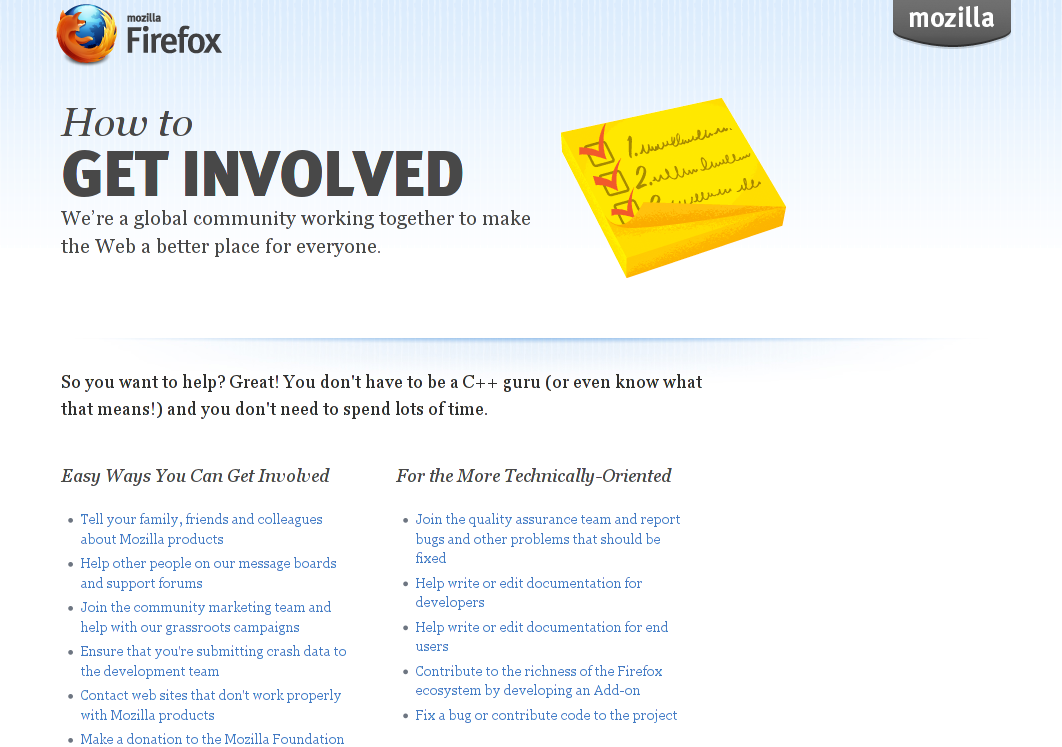
\includegraphics[height=0.8\textheight]{../img/mozilla-get-involved}

    \href{http://www.mozilla.org/en-US/firefox/community/}{http://www.mozilla.org/en-US/firefox/community/}
  \end{center}
\end{frame}

\begin{frame}
  \frametitle{How?}
  \begin{itemize}
    \setlength{\itemsep}{2em}
  \item \begin{LARGE} \textcolor{beamer@mygrey}{Contribute} \end{LARGE} \\ \textcolor{beamer@mygrey}{(to existing projects)}
  \item \begin{LARGE} \textcolor{beamer@myblue}{Create} \end{LARGE} \\ \textcolor{beamer@myblue}{(your own projects and make them open source)}
  \end{itemize}
\end{frame}

\begin{frame}
  \frametitle{Create}
  \begin{LARGE}
    \begin{tabular}{r l}
      Q: & How does something become open source? \\
      \only<2>{A: & Attach a \textcolor{beamer@myblue}{license} and share it with others \\}
    \end{tabular}
  \end{LARGE}
\end{frame}

\begin{frame}
  \frametitle{Software}

  Lots of licenses to choose from\ldots

  \begin{description}
  \item[GPL] Is now, and will forever be free
  \item[BSD] Is free, but new versions don't have to be free too
  \item[Apache] Similar to BSD
  \end{description}

  Lots and lots more: IBM, Intel, MIT, Mozilla, Python, Microsoft, Sun, \ldots

\end{frame}

\begin{frame}
  \frametitle{How to use a Software License}
  \begin{enumerate}
  \item Find the license you want (decide how "free" you want it to be)
  \item Fill in the blanks with your software's title
  \item Attach and distribute the license with your software package
  \item ????
  \item Share!
  \end{enumerate}
\end{frame}

\begin{frame}
  \frametitle{How to use a Software License}
  GPL, Apache, BSD all have how-to guides and/or examples
  \begin{description}
  \item[GPL] \href{http://www.gnu.org/licenses/gpl-howto.html}{http://www.gnu.org/licenses/gpl-howto.html}
  \item[Apache] \href{http://www.apache.org/dev/apply-license.html}{http://www.apache.org/dev/apply-license.html}
  \item[BSD] \href{http://www.opensource.org/licenses/BSD-3-Clause}{http://www.opensource.org/licenses/BSD-3-Clause}
  \end{description}
\end{frame}

\begin{frame}
  \frametitle{Hardware}
  \begin{itemize}
  \item Historically have used Open Software licenses, despite differences between software and hardware
  \item Hardware-specific Open Hardware Licenses (OHL):
    \begin{description}
    \item[TAPR OHL] (Tucson Amateur Packet Radio)
    \item[CERN OHL] (European Organization for Nuclear Research)
    \end{description}
  \end{itemize}
\end{frame}

\begin{frame}
  \frametitle{Content}
  \begin{center}
    
\includegraphics[width=0.5\textwidth]{../img/cc}
  \end{center}
\end{frame}

\begin{frame}
  \frametitle{Content}
  % http://www.squidoo.com/cc-flickr
  \begin{center}
    \begin{large}Do anything you want with it \end{large}

    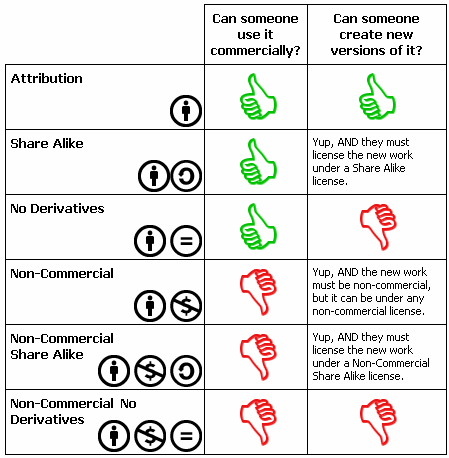
\includegraphics[height=0.7\textheight]{../img/cc-list}

    \begin{large}Copyright (\copyright) \end{large}
  \end{center}
\end{frame}

\begin{frame}
  \frametitle{How to use Creative Commons Licenses}

  Creative Commons has a guide to walk you through the process of generating a license you can attach to your content: \href{http://creativecommons.org/choose/}{http://creativecommons.org/choose/}

  \begin{center}
    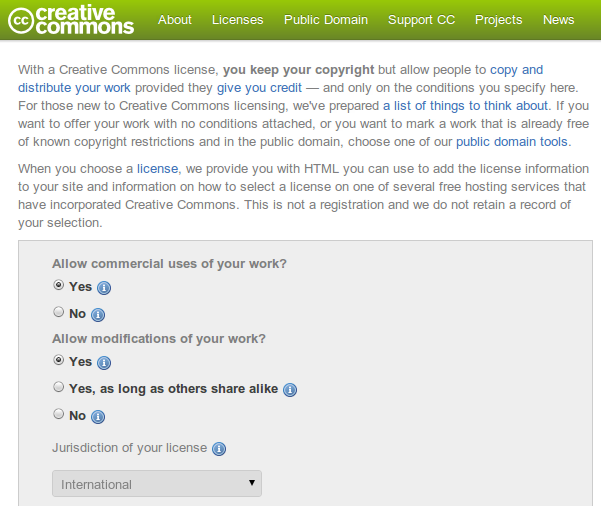
\includegraphics[height=0.7\textheight]{../img/cc-guide-short}
  \end{center}
  
\end{frame}

\begin{frame}
  \frametitle{How?}
  \begin{itemize}
    \setlength{\itemsep}{2em}
  \item \begin{LARGE} Contribute \end{LARGE} \\ (to existing projects)
  \item \begin{LARGE} Create \end{LARGE} \\ (your own projects and make them open source)
  \end{itemize}
\end{frame}

% http://news.ycombinator.com/item?id=3099362

\begin{frame}
  \frametitle{About Github...}
    \begin{Large}
      When it comes to hiring, I'll take a Github commit log over a
      resume any day.
      \begin{flushright}
        \textemdash{}John Resig
      \end{flushright}

    \end{Large}
\end{frame}

\begin{frame}
  \frametitle{Stuff you may not have learned in school}
  % \begin{overlayarea}{\textwidth}{\textheight}
    \begin{itemize}[<+->]
    \item Language: whatever the project is written in
    \item Build Process: Make, CMake autotools, Ant, Jam, Rake
    \item Version control: git, CVS, svn, Bazaar, Darcs, Mercurial
    \item Bug Trackers: Bugzilla, Trac, Mantis, Launchpad
    \item Communication: Forums, Wikis, IRC
    \item Source Code Communities: github, Bitbucket, Launchpad,
      Gitorious, Google Code, SourceForge
    \end{itemize}
  % \end{overlayarea}
\end{frame}

% http://www.kegel.com/academy/opensource.html
% http://stackoverflow.com/questions/43649/how-to-get-involved-in-an-open-source-project

\end{document}
